%!TEX root = ../thesis.tex
%*******************************************************************************
%****************************** Second Chapter *********************************
%*******************************************************************************

\chapter{Background}
\label{chapter2}

\ifpdf
    \graphicspath{{Chapter2/Figs/Raster/}{Chapter2/Figs/PDF/}{Chapter2/Figs/}}
\else
    \graphicspath{{Chapter2/Figs/Vector/}{Chapter2/Figs/}}
\fi

%********************************** %First Section  **************************************
\section{Lattice models}
\label{sec:lattice-models}

\subsection{Historical introduction}
\label{subsec:latt-hist}
\begin{itemize}
	\item I think starting from the magnetism point of view might be the best way to go, slowly lead into the field of condensed matter theory and lattice models. 
\end{itemize}

\subsection{The Schr{\"o}dinger equation and the Feynman path integral}
\label{subsec:latt-qm}
The wavefunction
\begin{equation}
	\Psi\left(r_{1}, \ldots, r_{N}\right)
\end{equation}
the Schr\" odinger equation
\begin{equation}
	i \frac{\partial \psi(\boldsymbol{r}, t)}{\partial t}= \hat{H} \psi(\textbf{r}, t)
\end{equation}
for a single particle in an external potential $\hat{V}(\boldsymbol{r})$ the Hamiltonian is 
\begin{equation}
	\hat H \phi(\boldsymbol{r})=-\frac{1}{2} \nabla^{2} \phi(\boldsymbol{r})+\hat{V}(\boldsymbol{r}) \phi(\boldsymbol{r}).
\end{equation}
Alternatively to the Schr\" odinger equation one can use an integral Green's function representation to express the wavefunction $\psi$ at some future time $t_2$ given initial condition $\psi(\boldsymbol{r}, t_1)$ as
\begin{equation}
	\psi\left(\boldsymbol{r}_{2}, t_{2}\right)=\int  \mathcal{K}\left(\boldsymbol{r}_{2}, t_{2} ; \boldsymbol{r}_{1}, t_{1}\right) \psi\left(\boldsymbol{r}_{1}, t_{1}\right) \mathrm{d} \boldsymbol{r}_{1}.
\end{equation}
The solution to  equation
\begin{equation}
	\left(i \frac{\partial}{\partial t_{2}}-H_{\boldsymbol{r}_{2}}\right) \mathcal{K}\left(\boldsymbol{r}_{2}, t_{2} ; \boldsymbol{r}_{1}, t_{1}\right)=i \delta\left(\boldsymbol{r}_{1}-\boldsymbol{r}_{2}\right) \delta\left(t_{1}-t_{2}\right)
\end{equation}
and the \textit{propagator} $\mathcal{K}\left(\boldsymbol{r}_{2}, t_{2} ; \boldsymbol{r}_{1}, t_{1}\right)$ is expressed using the Feynman path integral
\begin{equation}
	\label{eq:FPI}
	\mathcal{K}\left(\boldsymbol{r}_{2}, t_{2} ; \boldsymbol{r}_{1}, t_{1}\right)=\int_{\substack{\boldsymbol{r}\left(t_{1}\right)=r_{1} \\ \boldsymbol{r}\left(t_{2}\right)=r_{2}}}  \mathcal{D} \boldsymbol{r}(t) \exp \left(i \int_{t_{1}}^{t_{2}} \mathcal{L}(\boldsymbol{r}, \dot{\boldsymbol{r}}) d t\right),
\end{equation}
where $\mathcal{L}$ is the classical Lagrangian function of the system
\begin{equation}
	L(\boldsymbol{r}, \dot{\boldsymbol{r}})=\frac{1}{2} \dot{\boldsymbol{r}}^{2}-\hat V(\boldsymbol{r}),
\end{equation}
and the integral is over all paths that satisfy the endpoint conditions.

\subsection{Examples of lattice models}
\label{subsec:latt-examples}

\begin{equation}
	\hat{\sigma}^x_{i}=\left(\begin{array}{cc}0 & 1 \\ 1 & 0\end{array}\right)_{i} \quad \hat{\sigma}^y_{i}=\left(\begin{array}{cc}0 & -i \\ i & 0\end{array}\right)_{i} \quad \hat{\sigma}^z_{i}=\left(\begin{array}{cc}1 & 0 \\ 0 & -1\end{array}\right)_{i}
\end{equation}


\subsubsection{Transverse-field Field Ising model}
\begin{equation}
	\hat H_{\mathrm{Ising}}=-J \sum_{\langle i, j\rangle} \hat{\sigma}^z_{i} \hat{\sigma}^z_{j}-h \sum_{i} \sigma^x_{i}
\end{equation}

\subsubsection{Heisenberg model}
\begin{equation}
	\hat{H}_{\mathrm{Heisenberg}}=-\frac{1}{2} \sum_{j=1}^{N}
	\left[J_{x} \hat{\sigma}_{j}^{x} \hat{\sigma}_{j+1}^{x}+J_{y} \hat{\sigma}_{j}^{y} \sigma_{j+1}^{y}+J_{z} \hat{\sigma}_{j}^{z} \hat{\sigma}_{j+1}^{z}+h \hat{\sigma}_{j}^{z}
	\right]
\end{equation}

\subsubsection{Bose-Hubbard model}
\begin{equation}
	\hat{H}_{\mathrm{BH}}= -t \sum_{\langle i, j\rangle} \hat{b}_{i}^{\dagger} \hat{b}_{j}+\frac{U}{2} \sum_{i} \hat{n}_{i}\left(\hat{n}_{i}-1\right)-\mu \sum_{i} \hat{n}_{i}
\end{equation}

%********************************** % ??? Section  *************************************
\newpage
\section{Solutions to the many-body problem and QMC}
\label{sec:qmc}

\begin{itemize}
	\item Mention Complexity of QMC for fermions and bosons
	\item A more broad overview of methods that can be used for studying the many body problem (DRMG), with particular applications to lattice methods
	\item Partition QMC into nicer subsections
\end{itemize}

The Schr{\"o}dinger equation underpins a large part of quantum chemistry and solid state physics. However, the quantum many-body problem, which amounts to solving the $3N$-dimensional Schr\"odinger equation is notoriously hard to solve. Ever since the postulation of the equation in 1925, great efforts have been made in solving the equation, both analytically and numerically. Perhaps most impactful was the development of various approximate methods to solve the many-body problem with the available computational resources. Hartree-Fock (HF) approaches solve an auxiliary system of independent electrons in a self-consistent field and assume that the wave function (for fermions) can be represented as a single Slater determinant. The HF method does not include electron correlation, which makes it a good approximation only in systems where correlation contributions are small. Post-HF methods, such as Coupled Cluster, Configuration interaction and M\o ller-Plesset theory include correlation by considering a linear combination of determinants. They can be extremely accurate but come at a high computational cost. 

One of the most popular approaches used today is Density Functional Theory (DFT). It reformulates the many-body electron problem in terms of the $3$-dimensional electron density $n(\mathbf{r})$, which is found by minimising the total energy functional $E[n(\mathbf{r})]$~\cite{hohenberg1964inhomogeneous}. DFT provides an alternative line of thought to the truncated Hilbert space of single particle orbitals~\cite{kohn1999nobel} and is used extensively for simulating large systems as linear scaling variants of DFT exist~\cite{skylaris2005introducing}. 
While DFT is theoretically exact the true energy functional $E[n(\mathbf{r})]$ is not known and its parameterisations employ more accurate \emph{ab initio} methods. One of which being Quantum Monte Carlo (QMC).

\subsection{Overview}
\label{subsec:qmc-overview}
%% General about QMC
Quantum Monte Carlo is a class of methods that uses statistical sampling to directly deal with high-dimensional integration that arises from working with the many-body wave function. QMC methods are among the most accurate achieving chemical accuracy for smaller systems~\cite{foulkes2001quantum}, and can achieve any degree of statistical precision sought. Quantum Monte Carlo is also very versatile and can be applied at both zero and finite temperatures~\cite{austin2012quantum}.	
%% Zero temperature methods
%% Variational quantum monte carlo
The most basic zero temperature QMC method is variational QMC (VMC). The method is composed of two parts, firstly it directly evaluates the variational energy $E_V = \langle \Psi_{T} | \hat H | \Psi_{T} \rangle / \langle \Psi_{T} | \Psi_{T} \rangle$ of the system using Monte Carlo integration and a trial wave function $\Psi_{T}$. Secondly the parameters of the trial wave function are optimised such as to minimise the variational energy $E_V$, giving the method its name. The first application of VMC was to ground state ${}^4$He~\cite{mcmillan1965ground} and was later extended for studying many-body fermionic systems~\cite{ceperley1977monte}. A way of obtaining excitation energies using VMC is to use a trial wave function that models an excited state of the system, if the trial wave function obeys a certain symmetry, the variational principle guarantees that this VMC energy calculation gives an upper bound on the lowest exact eigenstate of this symmetry. Furthermore, the method can be extended to study non-equilibrium properties of bosonic~\cite{carleo2012localization, carleo2014light}, and fermionic~\cite{ido2015time} systems. The main advantage of VMC is its simplicity while the main drawback is that the accuracy is limited by the flexibility and form of the trial wave function~\cite{austin2012quantum}. As such VMC is usually employed as a first step in more advanced QMC simulations. 

%% Green function QMC and Diffusion QMC
Projector quantum Monte Carlo (PMC) is a class of QMC methods which are in essence nothing more than stochastic implementations of the power method to obtain the dominant eigenvector of a matrix or a kernel function~\cite{gubernatis_kawashima_werner_2016}. Their distinct advantage over VMC is that they are not constrained by our parametrisation of the trial wave function, as they can describe arbitrary probability distributions. The projector $\hat P$ has to be chosen in such a way, that the ground state of the system becomes the dominant eigenvector, i.e. $| \Psi_{0}\rangle = \lim_{n\rightarrow \infty} \hat{P}^n |\Psi_{T}\rangle$. Different ways of achieving this give rise to different flavours of PMC methods, e.g choice of space (real or orbital space) in which the walk is done and choosing either first or second quantisation. Using an exponential projector $\hat{P} = e^{\tau (E_T \mathbb{1} - \hat{H})}$ can be interpreted as propagation in imaginary time $\tau \rightarrow it$ in turn transforming the Schr\"odinger equation into a diffusion equation, which is a continuous limit of the random walk and lends itself to stochastic integration~\cite{reynolds1990diffusion}. Directly sampling from the exact Green function is known as Projector Green Function Monte Carlo (GFMC) method~\cite{kalos1962monte, kalos1966stochastic}. A convenient approximation to GFMC is its short-time approximation which leads to one of the most popular QMC methods, diffusion Monte Carlo (DMC)~\cite{foulkes2001quantum, reynolds1990diffusion}. In this regime one can exploit analytical solutions to diffusion and rate problems to write an explicit form of the Green's function. Additionally, by using the Trotter-Suzuki formula the time-step bias can be expressed and accounted for~\cite{austin2012quantum}. DMC is statistically implemented by using a population of walkers which either branch or die, over which the average is calculated. Reptation quantum Monte Carlo~\cite{reynolds1990diffusion} (RMC) is an alternative formulation which only uses a single walker, and instead of branching and dying the MC moves mutate the path of that single walker. The use of a guiding wave function for importance sampling greatly improves the statistical efficiency of PMC methods. The guiding wave function is usually obtained by means of VMC or some mean field calculation. 

PMC methods suffer from the \emph{sign problem}, which is present in Markov chain simulation of distributions that are not strictly positive, thus in fermionic and frustrated systems~\cite{gubernatis_kawashima_werner_2016}. The problem refers to an exponential decrease in sampling efficiency with system size. The search for solutions of this problem is still an area of active research~\cite{foulkes2001quantum} but is in practice remedied by the \emph{fixed-node} approximation~\cite{anderson1975random}. It imposes a boundary condition into the projection, such that the projected state shares the same zero crossings (nodal surface) with a trial wave function, which is again usually obtained with VMC. The projected state is now only exact when the nodal surface is exact. Nevertheless this approximation is quite accurate~\cite{foulkes2001quantum}. Fixed node is widely used, one of its first applications being the electron gas~\cite{ceperley1980ground}, which is used in parameterisations of the  exchange correlation functional in LSDA~\cite{vosko1980accurate}.

%% Finite temperature methods
Quantum Monte Carlo methods have had a lot of success at finite temperatures. Auxiliary-field Monte Carlo, or Path Integral Monte Carlo~\cite{ceperley1995path}, which leads to ring-polymer molecular dynamics, may be used for this purpose. Additionally QMC is not limited to continuum space applications and has been extensively used to study lattice models, notable examples being the cluster/loop algorithm and the worm algorithm~\cite{gubernatis_kawashima_werner_2016, prokof1998exact}.

%% Computational considerations
Quantum Monte Carlo methods are generally more computationally expensive than DFT approaches, but on the other hand QMC codes are, as a rule of thumb, simpler to implement. Furthermore, since the wave function does not need to be stored directly, QMC has reasonable storage requirements. The high computational cost of the QMC methods is remedied by the fact that they are intrinsically parallelisable, the core calculation involves generating (pseudo)-random numbers, performing a simple calculation and in the end averaging over the results. Therefore, implementations of QMC algorithms that have been applied to practical problems are optimised to run on massively parallel hardware with little overhead~\cite{needs2020variational}. Finally, the repetitive nature of the Monte Carlo calculation lends itself to hardware acceleration using either graphical processing units (GPUs) or field-programmable gate arrays (FPGAs)~\cite{austin2012quantum}.

%********************************** %???? Section  *************************************
\newpage
\section[The Feynman-Kac formula]{Feynman-Kac: connecting Quantum Mechanics and Stochastic Processes}
\label{subsec:FK}

\subsection{Stochastic processes}
\label{subsec:fk-stoch}


Introduce minimal necessary basics to understand the following section/discussions. This includes
\begin{itemize}
	\item Random variables
	\item Markov processes, Markov process generator
	\item Wiener process
	\item 
	\item Master equation, Transition matrices and Fokker-Plank, Fokker-Planck generator?
\end{itemize}

\subsubsection{Master equation}
Describes the time evolution of a system which can be described as a probabilistic combination of states and the transitions between these states is encapsulated with the \emph{transition rate matrix}.
\begin{equation}
	\partial_{t} \mathbf{P} = A \mathbf{P},
\end{equation}
where $A$ are the \emph{connections} and $\mathbf{P}$ are the probabilities.  

\subsection{Feynman-Kac formula}
\label{subsec:fk-fk}
The Feynman path integral formulation~\eqref{eq:FPI} was extensively used by physicists for decades, even in the absence of a formal mathematical formulation which is hard to define because of the difficulties with defining an appropriate measure on the path space. Kac~\cite{kac1949distributions} provided a rigorous formulation of the \textit{real-valued} case of the Feynman path integral, and the resulting \emph{Feynman-Kac} formula provides a bridge between \emph{parabolic} partial differential equations and stochastic processes.

To illustrate the Feynman-Kac formula let us consider a single particle with Hamiltonian
\begin{equation}
	\hat{H} = -\frac{\mathrm{d}^2~~}{\mathrm{d}x^2} + V(x)
\end{equation}
and the Schr\" odinger equation in \textit{imaginary time}, which is of the elliptic type, 
\begin{equation}
	\label{eq:imag_sch}
	\partial_t | \psi_t \rangle = - \hat{H} | \psi_t \rangle.
\end{equation}
Its formal solution, the time propagation of an initial wave function $|\phi_0\rangle$ at $t=0$, is written as
\begin{equation}
	\left| \psi_{t} \right\rangle = e^{-\hat{H} t}\left|\psi_{0}\right\rangle. 
\end{equation}
From the spectral decomposition of the operator $e^{-\hat{H} t}$ in terms of eigenstates $|\phi_n\rangle$ and eigen-energies $E_n$ of the Hamiltonian $\hat{H}$
\begin{equation}
	e^{-\hat{H} t}=\sum_{n} e^{-E_{n} t}|\phi_n\rangle\langle\phi_n|, 
\end{equation}
it follows that the term corresponding to the ground state of the system $|\phi_0\rangle$ decays the slowest. Thus starting in some initial state and propagating for a long imaginary time $it$ leads into the ground state with the decay rate giving the ground state energy as
\begin{equation}
	\lim_{t \rightarrow \infty} | \psi_t \rangle \propto e^{-E_0 t} | \phi_0 \rangle,
\end{equation} 
where $E_0$ is the ground state energy and $|\phi_0\rangle$ is the corresponding state. Kac noticed that the kinetic term of the Lagrangian in~\eqref{eq:FPI} could be interpreted as a measure on Brownian walks, and a solution to the imaginary time Schr\" odinger equation can be written as
\begin{equation}
	\psi(x, t)=\underset{X \sim \text { Brownian with } X_{t}=x}{\mathbb{E}}
	\left[\exp \left(-\int_{0}^{t}  V\left(X_{\tau}, \tau \right) \mathrm{d}\tau \right) \psi\left(X_{0}, 0\right)\right],
\end{equation}
where only the \textbf{endpoint} at time $t$ of the Brownian process fixed, whereas the starting point at time $t=0$ is not, $\psi (x, 0)$ encodes the initial condition into this representation. When there is no external potential $V(x) = 0$, the Schr\" odinger equation in imaginary time is the diffusion equation and the Feynman-Kac solution is simply
\begin{equation}
	\begin{aligned} 
		\psi(x, t) &= \underset{X \sim \text { Brownian with } X_{t}=x}{\mathbb{E}}\left[\psi\left(X_{0}, 0\right)\right] \\
		&=  
		\frac{1}{\sqrt{2 \pi t}} \int  e^{-\left(x-x^{\prime}\right)^{2} / 2 t} \psi_{0}\left(x^{\prime}\right) \mathrm{d} x^{\prime}
	\end{aligned}
\end{equation}
An illustration of the Feynman-Kac approach to the problem with no external potential $V(x)$ in 1D is depicted in Fig.~\ref{fig:fk_1d_example}.
\begin{figure}[H]
	\centering
	\subfloat
	{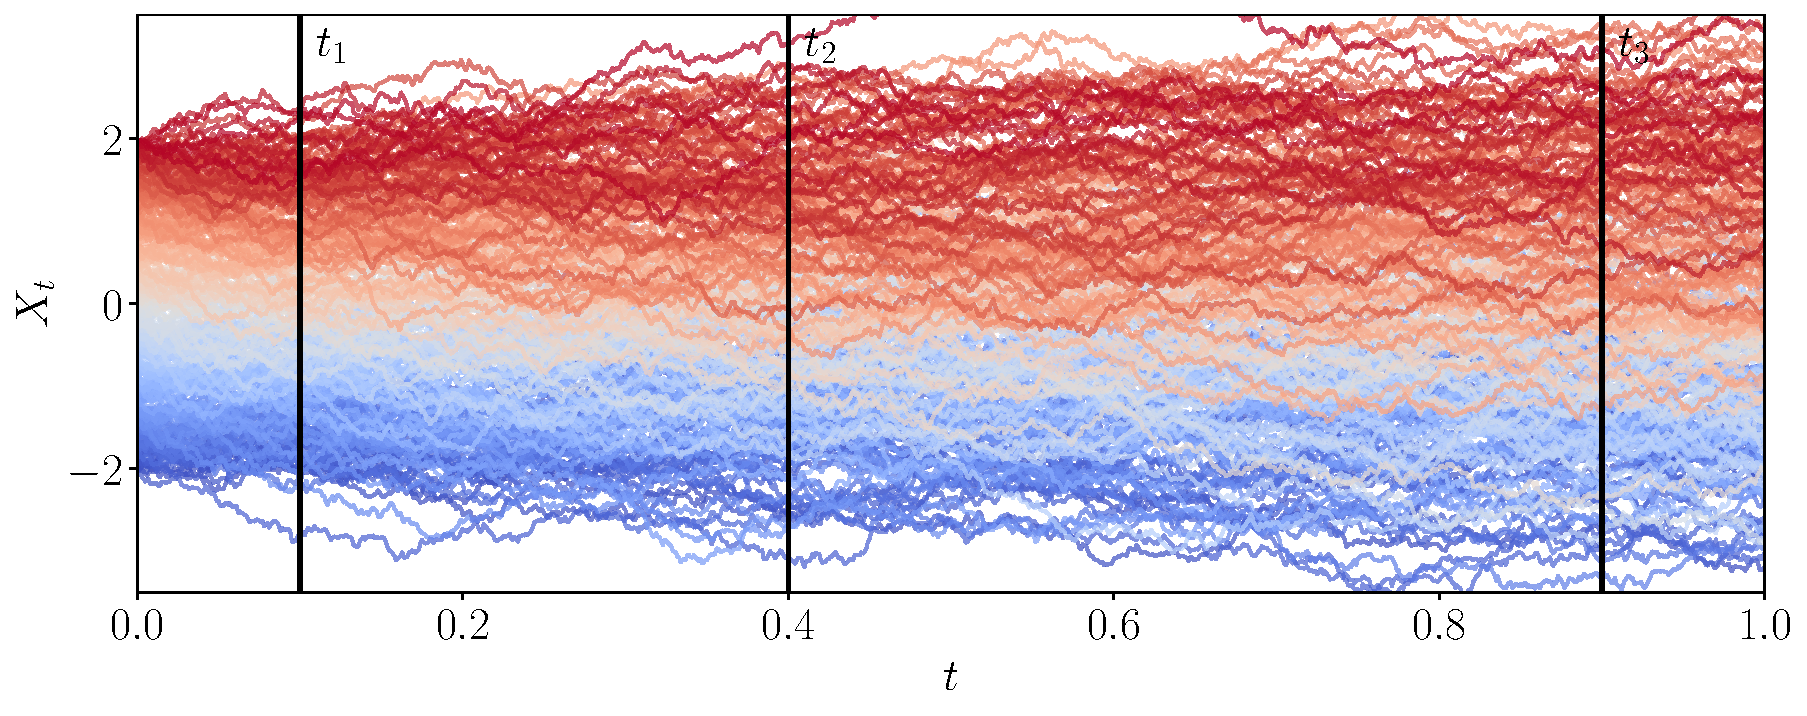
\includegraphics[width = \linewidth]{Chapter2/Figs/Raster/fkac_vs_fplanck_top.pdf}} \\
	\subfloat
	{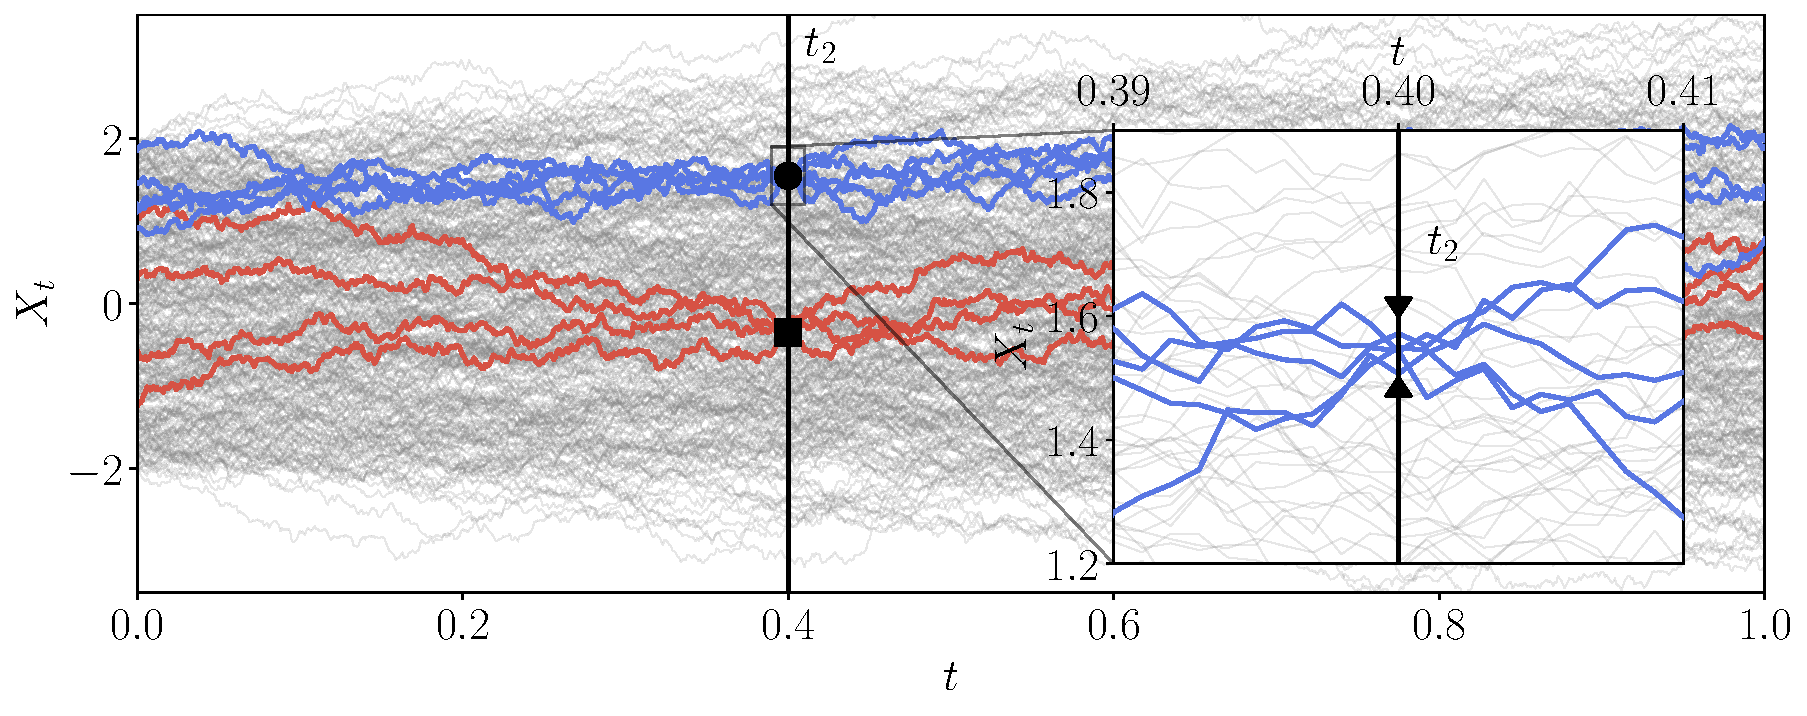
\includegraphics[width = \linewidth]{Chapter2/Figs/Raster/fkac_vs_fplanck_mid1.pdf}} \\
	\subfloat
	{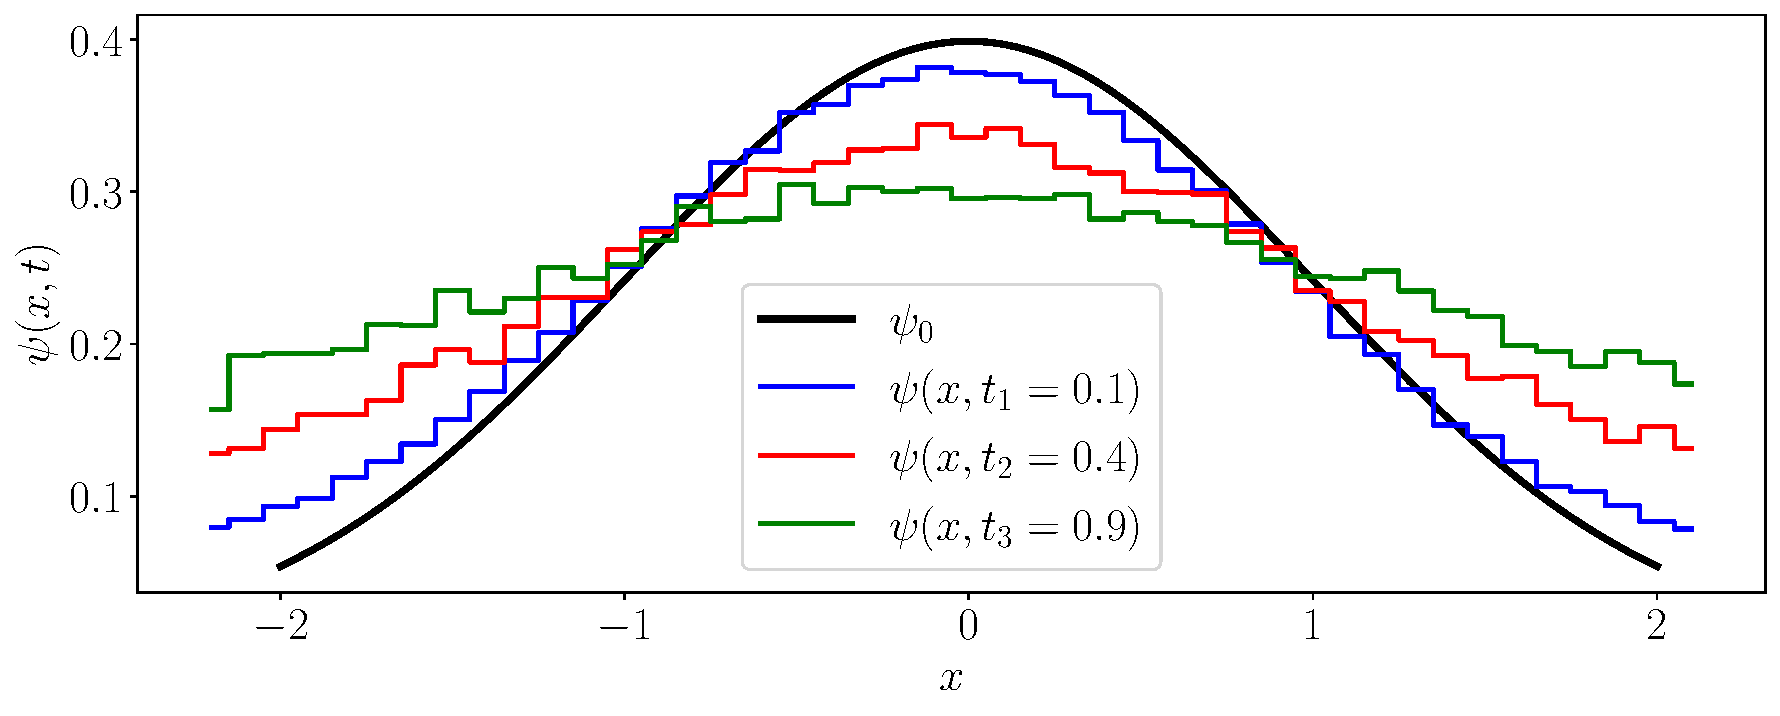
\includegraphics[width = \linewidth]{Chapter2/Figs/Raster/fkac_vs_fplanck_bottom.pdf}}
	
	\caption[Feynman-Kac for a 1D free particle]{\textbf{Feynman-Kac for a 1D free particle.} \textbf{top:} $N=400$ Brownian walks starting from different $x_0$, the color signifies initial position. In order to evaluate $\psi$ between $x-\frac{\delta x}{2}$ and $x+\frac{\delta x}{2}$ at some time $t$ we must first find Brownian paths that end there. \textbf{middle:} The paths that pass through at $x \in (1.5, 1.6)$ (blue) and through $x \in (-0.4,-0.3)$ (red) are colored, others are left in grey. \textbf{bottom:} Time evolution of the initial condition $\psi_{0} = \frac{1}{\sqrt{2 \pi}} e^{-\frac{1}{2} x^{2}}$, by estimating ${\mathbb{E}}\left[\psi\left(X_{0}, 0\right)\right]$ from the filtered paths at each timestep.}
	\label{fig:fk_1d_example}
\end{figure}
This simple case, does not involve the potential $V(x)$. The role of the potential in the Feynman-Kac formula is to weight the Brownian paths, in turn defining the Feynman-Kac \emph{path measure} $\mathbb{P}_{\mathrm{FK}}$. A path measure is simply a measure on the path space and the Feynman-Kac measure is related to the Brownian measure $\mathbb{P}_{0}$ by the \emph{Radon-Nykodym} derivative
\begin{equation}
	\frac{\mathrm{d} \mathbb{P}_{\mathrm{FK}}}{\mathrm{d} \mathbb{P}_{0}}=\mathcal{N} \exp \left(-\int V\left(X_{t}\right) d t\right),
\end{equation}
where $\mathcal{N}$ is a normalizing constant. Intuitively we can understand the measure as assigning more weight to Brownian paths that spend more time in the attractive region ($V(x) < 0$) than in repulsive regions ($V(x) > 0$), this is illustrated in Fig.~\ref{fig:fkac_measure_reweight}.
\begin{figure}[H]
	\centering
	\subfloat{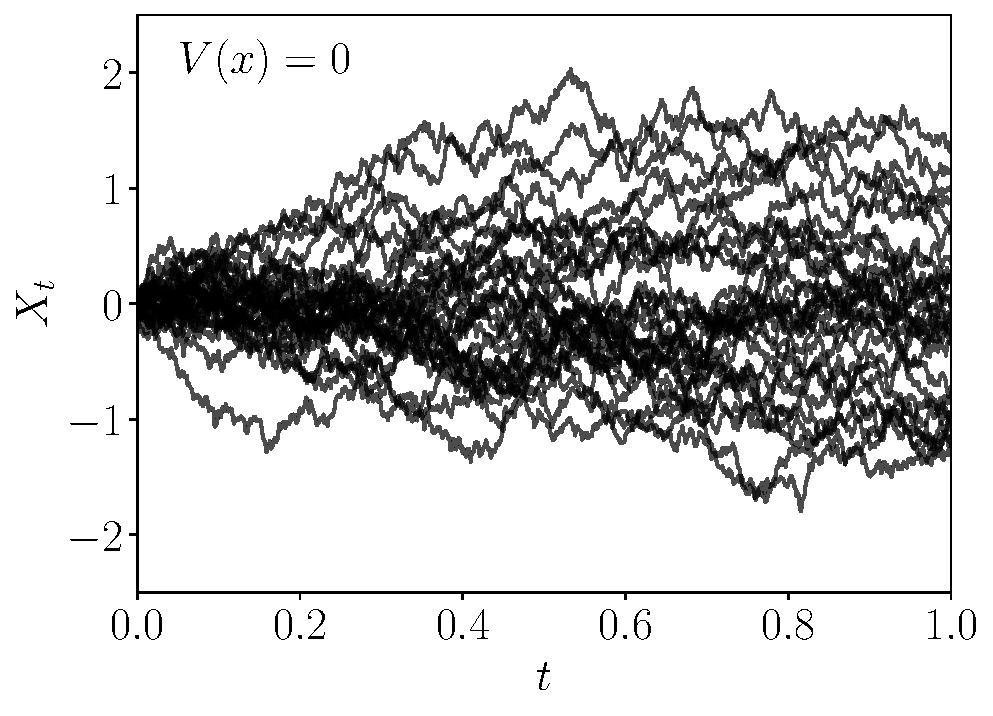
\includegraphics[width=0.5\linewidth]{Chapter2/Figs/Raster/reweight1.pdf}}
	\subfloat{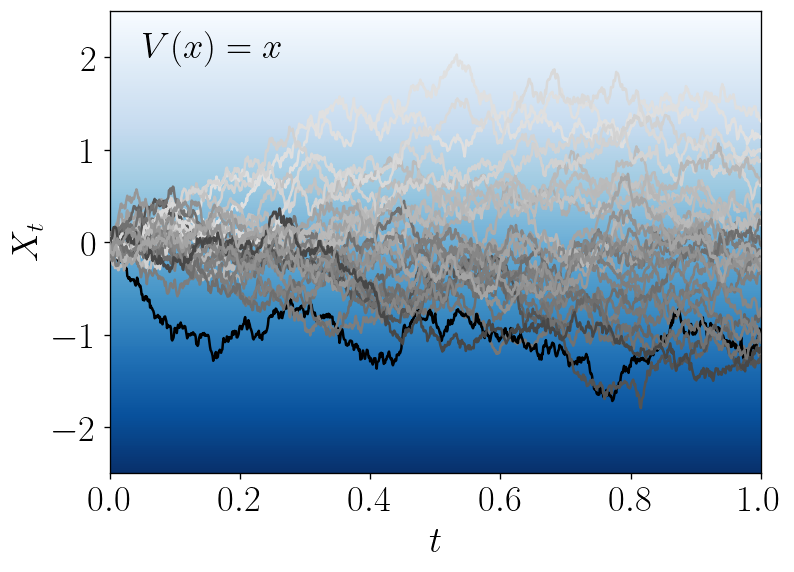
\includegraphics[width=0.5\linewidth]{Chapter2/Figs/Raster/reweight2.png}}
	\caption[Feynman-Kac measure in a linear potential]{\textbf{Feynman-Kac measure in a linear potential.} 
	\textbf{left:} $N=30$ Brownian paths. \textbf{right:} The paths colored by their likelihood under the Feynman-Kac measure with $V(x)=x$. }
	\label{fig:fkac_measure_reweight}
\end{figure}
Moreover, this new stochastic process is Markovian. This is crucial for our approach because of the connection with SDEs. In the continuous case we have discussed so far, the mapping between the Fokker-Planck equation and the Schr\" odinger equation is straightforward in terms of a similarity transform. Starting from the FP equation with drift $v(x)=-U^\prime(x)$ given as a gradient of some potential function $U(x)$ and its solution $\rho(t, x)$ 
\begin{equation}
	\frac{\partial \rho}{\partial t}=\mathcal{L}_{\mathrm{FP}} \rho=\frac{\partial}{\partial x}\left[\frac{\partial \rho}{\partial x}+U^{\prime}(x) \rho\right],
\end{equation}
we can define the function 
\begin{equation}
	\psi(x, t)=\frac{\rho(x, t)}{\sqrt{\rho_{0}(x)}},
\end{equation}
with $\rho_{0}$ being the stationary distribution of the FP equation
\begin{equation}
	\frac{\partial}{\partial x}\left[\frac{\partial \rho}{\partial x}+U^{\prime}(x) \rho\right] = 0 \quad \rightarrow \quad \rho_{0}(x) \propto \exp (-U(x)).
\end{equation}
Function $\psi(x, t)$ satisfies the imaginary time Schr\" odinger equation~\eqref{eq:imag_sch} with the Hamiltonian
\begin{equation}
	H=-\frac{\partial^{2}}{\partial x^{2}}-\frac{U^{\prime \prime}}{2}+\frac{U^{\prime 2}}{4}, 
\end{equation}
its ground state wavefunction is 
\begin{equation}
	\psi_{0}(x)=\sqrt{\rho_{0}(x)}.
\end{equation}
In other words, the quantum ground state probability distribution $|\psi_{0}|^2$ is the same as classical stationary distribution $\rho_{0}$ of the stochastic process $X_{t}$
\begin{equation}
	\mathrm{d} X_{t}=\mathrm{d} W_{t}+v\left(X_{t}\right) \mathrm{d} t,
\end{equation}
in the literature referred to as the \emph{Nelson's ground state process}~\cite{nelson1967dynamical, albeverio1977energy}. \hl{This connection serves as the backbone of our solution approach (revisit)}, as the ability to efficiently sample from the stochastic process is equivalent to sampling from the ground state of the quantum system. Even though the connection is simple, it comes with a caveat. Starting from the Schr\" odinger equation one needs to find the drift $v(x)$ and while the connection with the potential of the Hamiltonian is clear-cut in 1D, this is not the case in many-body systems, i.e. the \emph{inverse problem} of finding the stochastic process of a given Hamiltonian is difficult, and is one of the core problems approached in this thesis.

\newpage
\subsection{Stoquastic Hamiltonians and Lattice-model representations}
\label{subsec:fk-latt}
A similar connection between stochastic processes and the ground state exists in the discrete space, the difference being that instead of FP we have the Master equation


For a Markov process over discrete states, we can write the master equation as 
\begin{equation}
	\frac{\partial P_{j}}{\partial t}=\sum_{k \neq j}\left[\Gamma_{k \rightarrow j} P_{k}-\Gamma_{j \rightarrow k} P_{j}\right].
\end{equation}





\subsubsection{Single Particle on a Lattice}
\begin{equation}
	\partial_{t} \psi_{j}=\frac{1}{2}\left[\psi_{j+1}+\psi_{j-1}-2 \psi_{j}\right]+V_{j} \psi_{j}
\end{equation}

\begin{equation}
	\psi_{j}(t)=\underset{X \sim \mathrm{SRW} \text { with } X_{t}=j}{\mathbb{E}} \left[\exp \left(-\int_{0}^{t}  V\left(X_{\tau}, \tau\right) \mathrm{d} \tau \right) \psi_{X_{0}}(0)\right]
\end{equation}

\subsubsection{Transverse-field Ising model}

\subsubsection{Heisenberg model}
Heisenberg ferromagnet
\begin{equation}
	\hat H_{\mathrm{F}}=-\frac{1}{2} \sum_{j}\left[\hat{\sigma}_{j}^{x} \hat{\sigma}_{j+1}^{x}+\hat{\sigma}_{j}^{y} \hat{\sigma}_{j+1}^{y}+\hat{\sigma}_{j}^{z} \hat{\sigma}_{j+1}^{z}\right]
\end{equation}

The XY model.
\begin{equation}
	\begin{aligned} 
		\hat H_{X Y}=-\sum_{j}\left[\hat{\sigma}_{j}^{x} \hat{\sigma}_{j+1}^{x}+\hat{\sigma}_{j}^{y} \hat{\sigma}_{j+1}^{y}\right] &=H_{\mathrm{F}}+\frac{1}{2} \sum_{j} \hat{\sigma}_{j}^{z} \hat{\sigma}_{j+1}^{z} \\ 						&=-\mathcal{W}+\sum_{j}\left[n_{j}\left(1-n_{j+1}\right)+n_{j+1}\left(1-n_{j}\right)\right] 
	\end{aligned}
\end{equation}

\begin{equation}
	\psi_{s_{1: N}}(t)=\underset{\Sigma_{[0, t]} \sim \operatorname{SEP} \text{ with } \Sigma_{t}=s_{1: N}}{\mathbb{E}}
\left[\exp \left(-\int_{0}^{t} d t^{\prime} \sum_{j}\left[n_{j}\left(1-n_{j+1}\right)+n_{j+1}\left(1-n_{j}\right)\right]\right) \psi_{\Sigma_{0}}(0)\right]
\end{equation}

\subsubsection{Bose-Hubbard model}

%********************************** % ??? Section  *************************************
\newpage
\section{Quantum Mechanics, Control and loss functions}

\subsection{Continuous space}

\subsection{Discrete space}

\begin{figure}
	\centering
	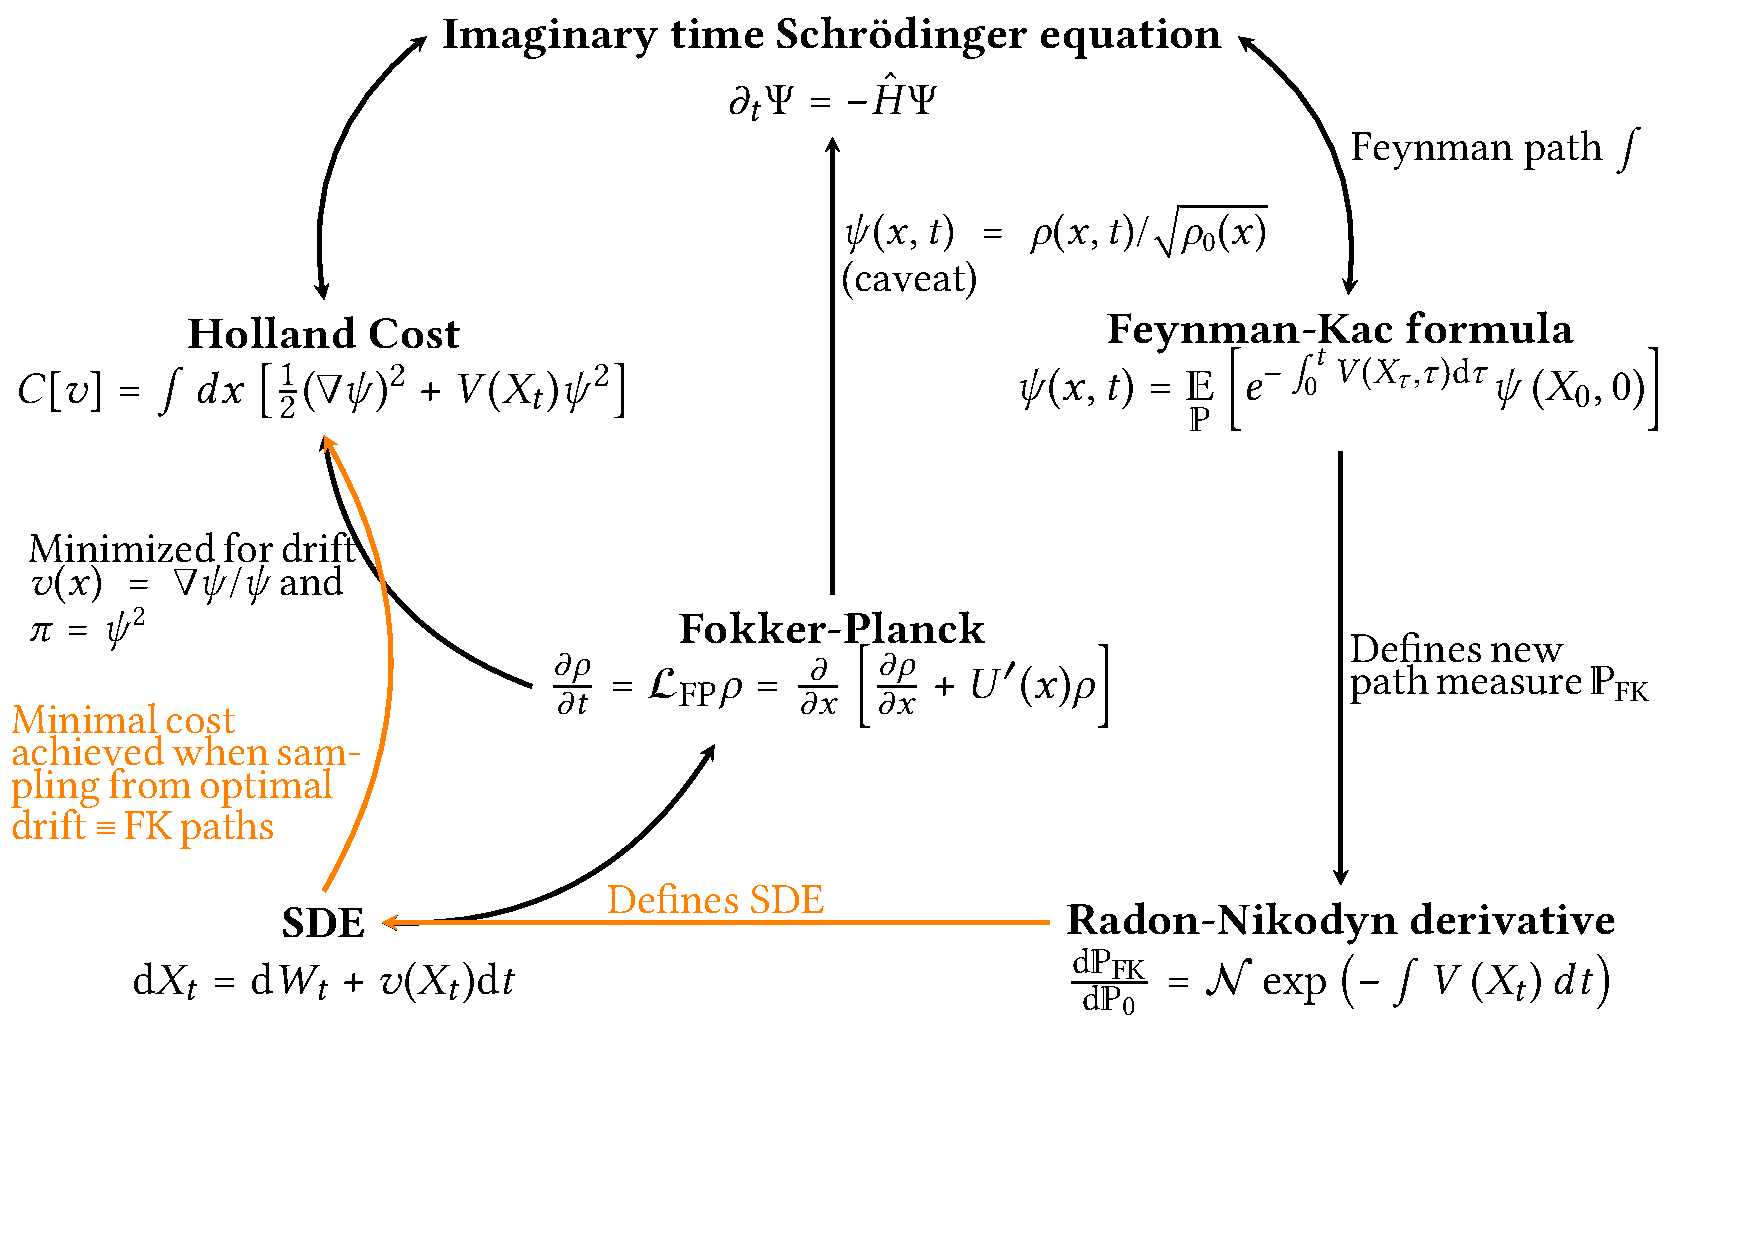
\includegraphics[angle=90, width=\linewidth]{Diagrams/bp/bp-c5}
	\caption[QM, stochastic processes and optimal control]{\textbf{QM, stochastic processes and optimal control}}
	\label{fig:bp-c5}
\end{figure}



%********************************** % ??? Section  *************************************
\newpage
\section{Machine Learning}
\label{sec:ml}

\subsection{Overview of ML approaches to the Quantum many-body problem}
\label{subsec:ml-overview}

\subsubsection{Neural Network Ansatzes}
\begin{itemize}
	\item
	\item
	\item
	\item
\end{itemize}

\subsection{Neural Networks}

\subsubsection{Convolutional Neural Networks}
\label{subsubsec:ml-cnn}

%********************************** % Ch2 Nomenclature *************************************
\nomenclature[z-sde]{SDE}{Stochastic Differential Equations}
\nomenclature[z-fp]{FP}{Fokker-Planck}
